% \section{Sequenzierungsbasierter Algorithmus}
% \subsection{Einführung}
% Der zweite Algorithmus stammt aus dem Bereich der Sequenzierung, genauer der Gensequenzierung. Gurundlage hierfür ist das Problem zwei (wahrscheinlich) ähnliche Genome zu vergleichen. Dafür muss eines der beiden bereits aufgeschlüsselt sein. Man nimmt dafür ähnliche Abschnitte der Genome zusammen, d.h. eine Folge  ist 'ähnlich' zu einer Folge im zweiten Genom (im Originalen Teilfolgen, aber für diese Arbeit reicht es nur Folgen zu betrachten). Alle solche Folgen werden als Paar abgespeichert. Ohne weitere Einschränkung seien die zu vergleichenden Folgen identisch.\\
% Wenn man nun diese Paare als Rechteckte im Raum annimmt (Start- und Endpunkte der Folgen sind jeweils die Ecken) wird nach einer Folge an Rechtecken gesucht, die nicht überlappend sind und der Weg sich immer nach oben rechts bewegt (vgl. Abbildung), dessen Gewichtung am größten ist.

% %Abbildung einfügen

% \subsection{Herleitung}
% Man sieht hier schon zwei parallelen zum HIS Problem. Einererseits ist eine aufsteigende Sequenz gesucht, andererseits haben diese Rechtecke auch eine Gewichtung, denn man möchte so wenig wie möglich aufschlüsseln müssen des zewiten Genoms. Problem ist jedoch die 2-Dimensionalität des Problems. Im folgenden wird eine Abwandlung zum Lösen des Ausgangproblem erklärt, welche die Dimension verringert und mit geschickter Gewichtung und Ordnung das HIS Problem löst. Die Ordnung ist im Folgenden als Priorität bezeichnet.\\
% Als Gewichtung nehmen wir hier die Länge der Folge an, die das Rechteck widerspiegelt. Da die Folgen identisch sind, handelt es sich um Quadrate mit der Länge $s$. Eine direkte Möglichkeit zum finden einer optimalen Folge wäre:\\
% \[
%     g.score=g.weight+max\{f.score | f \ll g\}
% \]

% Dieser Ansatz kann als Grundlage eines Dynamischen Algorithmus dienen, indem man die Quadrate anhand ihrer Startpunkte sortiert. Man sieht recht schnell, dass dies dem Algorithmus aus Kapitel 3 ähnelt in der Idee, denn $f\ll g$ ist vergleichbar mit dem Ansatz, das größte Element zu finden, welches um das Aktuelle erweitert werden kann ($prev$).\\

% \subsubsection*{Optimierung}
% Das ganze kann aber optimiert werden, in dem man sich Eigenschaften der Quadrate im Raum zu Nutze macht. Wenn man die x-Achse von 0 aus nach rechts entlang läuft und sich bei jedem Punkt $a$ anschaut welches die größte bisherige Folge ist, kann man die Quadrate $(s,t)$, die schon abgegangen sind, markieren. Alle diese Quadrate haben $t_1 < a$, die x-Koordinate von $t$ ist kleiner als $a$. $s$ ist also in der Berechnung nicht relevant und damit ist eine Dimension weniger nötig für die Berechnung. \\ Wir betrachten also die y-Koordinaten der Endpunkte aller Quadrate. Nehmen wir nun $(p,v)$ als Koordinaten an, p ist die Priorität (Die Position in der Ausgangsliste) und v ist die y-Koordinate des Endpunkts welche in dem Fall auch die Gewichtung widerspiegelt. Mit diesen Koordinaten bauen wir einen abgewandelten PST auf. Wie genau dieser erstellt wird, ist im Kapitel zur Implementierung beschrieben, wichtig ist aber folgende Eigenschaft hier: Die Blätter sind die Koordinaten. Von links nach rechts gelesen ist es wie in der gegeben Reihenfolge, d.h. das i-linkste Blatt ist das i-te Element $(i,v_i)$. Die inneren Knoten haben eine Priorität von $-\infty$ zu beginn (das ändert sich im Verlauf des Algorithmus') und dienen zum schnelleren finden folgendem Elementes: In einem Bereich von $(0,q)$ soll der Knoten gefunden werden, welcher den größten Score (Größte Summe an Gewichtungen) hat. Dies wird als $RMaxQ(0,q)$ bezeichnet. Da dies ein Blatt sein muss werden in den inneren Knoten diese geschickt gespeichert um schneller an dieses zu gelangen.\\
% An einem inneren Knoten $q$ ist $q.L$ bzw. $q.R$ der linke (rechte) Teilbaum. $q.Cv$ ist die Menge aller Blätter unter $q$ und $q.Pv$ ist das Blatt mit dem größten Score welches nicht in einem Knoten unter $q$ als $Pv$ gespeichert ist (vgl. Abbildung). $q.Hv$ ist das Schwerste Element aus $Cv$.


% \subsubsection*{Berechnung}
% Wenn man jetzt die optimale Folge an Rechtecken will, benötigen wir eine Möglichkeit das Quadrat kleiner dem Punkt $a$ zu finden, welchen den größten Wert hat. Im PST wird dies mit $RmaxQ(0,a)$ gemacht. Genauer wird darauf in Kapitel 6 eingegangen. Wenn dieser Wert gefunden wurde, muss nur noch das Quadrat an der Stelle $a$ angepasst werden um den neuen Wert. Dies wird gemacht in dem der Score geändert und dann ein Durchlauf durch alle Knoten gemacht wird. Dieser Vorgang entspricht dem Einfügen eines neuen Elementes in einer PQ, es wird aber kein Element direkt eingefügt, sondern ein Wert angepasst und dann die Integrität der Datenstruktur widerhergestellt. Auch werden nicht direkt Elemente getauscht, sondern nur die Werte in den Elementen. Dabei wird der abzugehende Teilbaum anhand von $a<h_{v.L}$ bestimmt.

% \subsection{Anpassen an das HIS}
% Wir haben also eine Liste an \an. Als priority nehmen wir die Position der Zahl und als key value den Wert der Zahl. Damit kann dann ein PST aufgestellt werden, welcher nach einem durchlauf von der Liste den Wert der HIS in sich hat am größten Blatt. Ein vereinfachter Pseudocode sieht wie folgt aus:

% \begin{lstlisting}[mathescape]
% his($a_n$)
% {
%     //Wurzel des Baumes
%     root =buildPST($a_n$); 
%     for(i = 1;i <= n; i++)
%     {
%         q = RMaxQ(0,$a_i$);
%         if(q.priority = $-\infty$)
%             continue;
%         root.CV[i].score +=q.score;

%         //Pv neu setzen im Baum
%         updatePv();
%     }
% }
% \end{lstlisting}

% Dieser Peusocode wirkt kurz, ist aber in der Implementierung aufwändiger als der erste Algorithmus.




\section{HIS als Sonderfall des Genomvergleichs \cite{ohlebusch}}

Dieses Kapitel führt das Problem des Genomvergleichs ein, ein Problem aus der Bioinformatik. Kern des Problems ist es zwei Genomen ($\sim$ Zeichenketten), in denen gemeinsame $"$ähnliche$"$ Abschnitte bekannt sind, diese gegenüberzustellen und eine größte Zuordnung zu finden, welche die originale Ordnung der Abschnitte beibehält. Wie festgestellt wird, ob die Abschnitte ähnlich sind, ist für den Algorithmus nicht relevant. 

\subsection{Herleitung}
Betrachtet man zwei Genome $G_1=a_1\dots a_n$ und $G_2=b_1\dots b_m$ über einem Alphabet $\Sigma$, sind zwei Abschnitte $A_1$ und $A_2$ lückenlose Bereiche aus $G_1$ und $G_2$, d.h. es existieren $i,j$ mit $1\leq i \leq j \leq n$ und $k,l$ mit $1\leq k \leq l \leq m$, s.d. $A_1 = a_i\dots a_j$ und $A_2 =b_k \dots b_l$. Man kann diese $"$Übereinstimmung$"$ durch ein Rechteck $R_1=((i,j),(k,l))$ charakterisieren. Man erhält dann eine Menge an Rechtecken $R$, welche alle ähnlichen Abschnitte enthält. Zusätzlich gibt es eine Funktion $f:R \mapsto \mathbb{N}$, welche jedem Abschnitt ein Gewicht ($weight$) zuordnet. Gesucht ist die Teilmenge $C \subset R$, für die die Summe aller Gewichte maximal ist. Zusätzlich dürfen zwei Rechtecke $R_x,R_y \in C$ nicht überlappend sein, also $R_x \ll R_y$ oder $R_y \ll R_x$ muss gelten. Zusätzlich wird ein Wert $score$ für jedes Rechteck $R_i$ gespeichert, welches am Ende für die Menge $R'=\{r | r \ll R_i\} \cup \{R_i\}$ die größtmögliche Summe der Gewichte nach vorheriger Anforderung abspeichert. Anschaulich bedeutet das, dass für ein Rechteck alle anderen Rechtecke betrachtet werden, welche nicht überlappend sind. Von denen wird das mit dem größten Score gewählt und mit $R_i$ erweitert.\\
Dies kann man als rekursive Gleichung formulieren:
\[ R_i.score =  R_i.weight + max\{r.score | r \ll R_i\}\]

\newtheorem{bemerkung}{Bemerkung}
\begin{bemerkung}[Parallele zum ersten Algorithmus]
Schon hier ist die Parallele zum ersten Algorithmus ersichtlich, $max\{r.score | r \ll R_i\}$ ist übertragbar auf $prev$ aus Kapitel 3. Genauso ist hier auch erkennbar, dass man für eine Menge an Rechtecken $R$ mit den Elementen $R_1 \dots R_n$ die obige Gleichung nur Anwenden kann, wenn\\ $max\{r.score | r\ll R_i\}$ bekannst ist, d.h. konkret, dass man für alle $r \ll R_i$ schon den $score$ berechnet haben muss. Also hat der $\ll$-Operator inherent eine Ordnung, nach welcher die Berechnung erfolgen muss. 
\end{bemerkung}


\subsection{erste Formulierung eines Algorithmus'}

\begin{definition}[$RMaxQ$ als Äquivalent zu $prev$] $prev(L,i)$ gibt, falls existent, das größtmögliche Element $y\in L$ zurück, mit $y\leq x$. Dies erweitern wir, indem wir in einem bestimmten Bereich $[a,b]$ das Rechteck mit dem größten $score$ haben wollen. Das bezeichnen wir als $RMaxQ(a,b)$. Im Falle $a=0$ bedeutet dies den Ursprung $(0,0)$.
\end{definition}

Anhand dieser Definition formulieren wir folgende Aussage:
Seien $G_1$ und $G_2$ Genome, $R_1, \dots, R_n$ ähnliche Abschnitte. Für ein $R_i=(s_i,t_i)$ mit $R_j=RMaxQ(0,s_i -(1,1))$ gilt $R_i.score=R_i.weight+R_j.score$. Das bedeutet, dass das Rechteck, welches $RMaxQ(0,s_i-(1,1))$ zurückgibt, auch $max\{r.score | r << R_i\}$ entspricht. Dies gilt per Definition von $RMaxQ(a,b)$,  da für $RMaxQ(0,s_i-(1,1))$ alle Rechtecke angeschaut werden, die vor $R_i$ kommen. Ein erster Algorithmus für das Problem sortiert $R_1,\dots ,R_n$ nach der $x_1$ Koordinate im Start- und Endpunkt und findet anhand dieser Ordnung $RMaxQ(0,R_i-(1,1));$
\begin{lstlisting}[mathescape]
GenomeAlignment(R){
    R=R.sort; //Sort w.r.t. $x_1$ coordinate
    for(i=1;i\leq n; i++){
        $R_j$=RMaxQ(0,$R_i$.s - (1,1));
        $R_i$.score=$R_i$.weight+$R_j$.score;
    }
    return RMaxQ(0,$R_n$.t);
}
\end{lstlisting}

\begin{bemerkung}[kleine Vereinfachung von $RMaxQ$]
Für diesen Algorithmus braucht man sowohl x- und y-Koordinate der Rechtecke, also zwei Werte. Durch die vorhin beschriebene Ordnung von $R_1 \ll \dots \ll R_n$, kann man das ganze verringern. Wir betrachten für $s_i=(x_i,y_i)$ (Den Startpunkt von $R_i$) die x-Koordinate $x_i$. Für diese gilt $x_1 < \dots < x_n$. Betrachten wir nun in der $i$-ten Iteration von $GenomeAlignment$ die Mengen $A=\{R_1,\dots , R_{i-1}\}$ und $I=\{R_i,\dots , R_n\}$. $A$ sind die schon betrachteten Rechtecke, und $I$ welche noch folgen. $RmaxQ(0,s_i-(1,1))$ schaut nur die Rechtecke in $A$ an. Zusätzlich gilt für alle $a \in A: a.s:=(x,y): x < x_i $. Die Startpunkte von allen Rechtecken in $A$ sind links vom Startpunkt von $R_i$. Somit ist die x-Koordinate der Startpunkte nicht mehr relevant, es reicht also eine alternative Definition $RMaxQ'(a,b)$ welche nur Zahlen keine Tupel bekommt, explizit hier $RMaxQ'(0,y_i-1)$.
\end{bemerkung}


\subsection{Anwendung auf den HIS}
Ein noch nicht betrachteter Sonderfall ist, wenn Start- und Endpunkt zusammenfallen, also für ein Rechteck $r=(s,t), s=t$ gilt. In diesem Fall sind die Rechtecke einzelne Punkte in der Ebene. Nun kann man für eine Folge \an ~die Folge an Paaren $(1,a_1),(2,a_2),\dots,(n,a_n)$~in der Ebene betrachten. Für $(i,a_i)$ ist $weight=a_i$.
\begin{center}
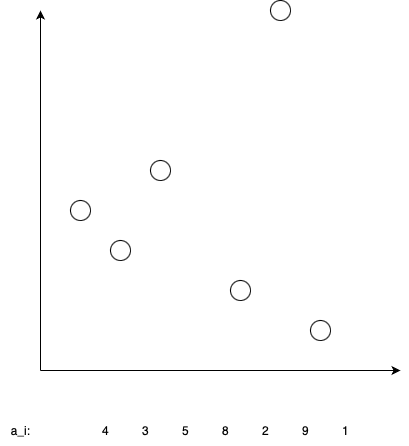
\includegraphics[scale=0.6]{./Pictures/HISGen.png}
\end{center}
\begin{bemerkung}[$RMaxQ(a,b)$ vs. $prev$]
$RMaxQ2(a,b)$ kann ein Rechteck mit Endpunkt $(\_,b)$ bestimmen (wie vorhin angemerkt, ist die x-Koordinate nicht relevant). Deshalb ist es nötig $RMaxQ(0,b-1)$ zu benutzen, $RMaxQ2(0,b)$ kann das Rechteck mit Endpunkt $(\_,b)$ zurückgeben, was offensichtlich nicht gewollt ist. Das bedeutet, dass $RMaxQ(0,b-1)$ äquivalent zu $prev(L,(\_,b))$ ist.  Da wir immer von $0$ ausgehen und nur schon betrachtete Werte in D sind, schreiben wir kurz $RMaxQ2(b)$.
\end{bemerkung}
Folgende Anpassung kann vorgenommen werden, um den Algorithmen an Punkte statt Rechtecke anzupassen:
\begin{lstlisting}[mathescape]
HIS($(a_n)$){
    L = (a_n).map(a_i -> (a_i,0); //Mapping a_i to (weight,score)
    A = new D; //initialising Data Structure D
    for(int i = 1; i \leq n ; i++){
       	q = RMaxQ2(a_i-1);
       	Prec[i] = q.i;
       	a_i.score=a_i.weight+q.score;
       	if(a_i.score > RMaxQ2(a_i).score)
       		insert(a_i);
       		while(a_i.score > next(a_i).score)
       			delete(next(a_i));
    }
}
\end{lstlisting}
\begin{small}
    Bemerkung: $next$ ist wie im Kapitel 2 zu verstehen.
\end{small}

Zum Rekonstruieren wird $Prec$ an der stelle $RMaxQ2(\infty).i$ durchgelaufen. Dies ist identisch zum Vorgehen aus Kapitel 3. Das folgende Unterkapitel beschäftigt sich mit der Frage, was die Unterschiede zwischen den Algorithmen sind und warum ein experimenteller Vergleich keine Aussagekraft über die Entscheidung hat, welcher Algorithmus besser in der Praxis ist.

\subsection{Vergleich}
Beide Algorithmen gehen nach dem gleichen Prinzip vor - das größte Erweiterbare Element zu finden, und dann erweitert einzusetzen. $prev$ und $RMaxQ$ sind in der Funktionsweise also äquivalent - unabhängig von der Datenstruktur. Genauso verwalten beide Algorithmen ein Array für die Rekonstruktion und löschen Elemente, die größer als $prev$ sind, aber im $score$ kleiner als das Neue. Der einzige fassbare Unterschied ist die Reihenfolge, also ob zuerst eingefügt, dann gelöscht wird, oder andersrum. Im Original vom Kapitel $4$ wird zusätzlich ein $(0,0)$ und $(\infty,\infty)$ eingefügt, damit nicht auf $\phi$ überprüft werden muss. Das ist aber eine Frage der Implementierung bzw. Programmierstil, und nicht des Algorithmus'.\\
$"$Note that the Algorithm 8.4 maintains the following invariant: If $q1 < q2 < ··· < ql$ are the entries in the data structure D, then $q1.score \leq q2.score \leq ··· \leq ql.score$.$"$\cite{ohlebusch}- dies beschreibt die Ordnung der Elemente in D. Interessanterweise können aber keine zwei Elemente mit gleichem $score$ in $D$ sein nach Zeile $8$ und $10$. Für den DP Algorithmus gilt $"$We maintain the invariant that L is strictly increasing in both coordinates. Therefore, the ordering based on their first coordinate (the alphabet ordering) can be used to order L. Figure 2 shows the HIS algorithm.$"$\cite{schensted1961longest}. Also auch eine strenge Monotonie der Elemente. Das bedeutet, dass die gleichen Elemente eingefügt und gelöscht werden müssen in einer Iteration, damit die Anforderungen erfüllt bleiben. Einzig in der Frage wie man mit einen Element, welches eingefügt werden soll, umgehen soll, dessen $score$ schon in $D$ Liste, unterscheiden sich die Algorithmen. Der DP Algorithmus löscht so ein Element und fügt das neue ein, dieser Algorithmus verändert D nicht. Wenn man im DP Algorithmus Zeile 15 in $if(v+a_i)\leq w$ umwandelt und in Zeile $16$ ein $continue$ statt $break$ hat, ergibt sich das gleiche Prinzip. Beide Algorithmen unterscheiden sich also minimal in der Vorgehensweise.\\
Da nach dem Gesetz der großen Zahlen es zufällig ist, wie der $score$ für ein Element aussieht, ist der Nutzen direkt abhängig davon, wie viele Elemente mit gleichem $score$ eingefügt werden. Man kann aber wie den DP Algorithmus auch diesen mit einem FT und kriegt dann einen abgewandelten Quellcode, der identisch dem vom DP Algorithmus ist. Die Laufzeitanalyse und Korrektheit ist nahezu identisch aus Kapitel 3 zu übernehmen.





 